% !TEX TS-program = XeLaTeX
% use the following command:
% all document files must be coded in UTF-8
\documentclass[spanish]{textolivre}
% build HTML with: make4ht -e build.lua -c textolivre.cfg -x -u article "fn-in,svg,pic-align"

\journalname{Texto Livre}
\thevolume{15}
%\thenumber{1} % old template
\theyear{2022}
\receiveddate{\DTMdisplaydate{2022}{7}{17}{-1}} % YYYY MM DD
\accepteddate{\DTMdisplaydate{2022}{7}{27}{-1}}
\publisheddate{\DTMdisplaydate{2022}{10}{13}{-1}}
\corrauthor{Karina Delgado Valdivieso}
\articledoi{10.35699/1983-3652.2022.40509}
%\articleid{NNNN} % if the article ID is not the last 5 numbers of its DOI, provide it using \articleid{} commmand 
% list of available sesscions in the journal: articles, dossier, reports, essays, reviews, interviews, editorial
\articlesessionname{dossier}
\runningauthor{Delgado Valdivieso y Jadan Guerrero} 
%\editorname{Leonardo Araújo} % old template
\sectioneditorname{Daniervelin Pereira}
\layouteditorname{Leonado Araújo}

\title{La neurodidáctica: una experiencia en educación inclusiva aplicada a las TIC}
\othertitle{Neurodidática: uma experiência em educação inclusiva aplicada às TIC}
\othertitle{Neurodidactics: an experience in inclusive education applied to ICT}
% if there is a third language title, add here:
%\othertitle{Artikelvorlage zur Einreichung beim Texto Livre Journal}

\author[1]{Karina Delgado Valdivieso \orcid{0000-0001-7459-1905} \thanks{Email: \href{mailto:karinadelgado@uti.edu.ec}{karinadelgado@uti.edu.ec}}}
\author[2]{Janio Jadan Guerrero  \orcid{0000-0002-3616-2074} \thanks{Email: \href{mailto:janiojadan@uti.edu.ec}{janiojadan@uti.edu.ec}}}
\affil[1]{Universidad Tecnológica Indoamerica, Facultad de Ciencias Humanas, de la Educación y Desarrollo Social, Ecuador.}
\affil[2]{Universidad Tecnológica Indoamerica, Centro de Mecatrónica y Sistemas Interactivos, Ecuador.}

\addbibresource{article.bib}
% use biber instead of bibtex
% $ biber article

% used to create dummy text for the template file
\definecolor{dark-gray}{gray}{0.35} % color used to display dummy texts
\usepackage{lipsum}
\SetLipsumParListSurrounders{\colorlet{oldcolor}{.}\color{dark-gray}}{\color{oldcolor}}

% used here only to provide the XeLaTeX and BibTeX logos
\usepackage{hologo}

% if you use multirows in a table, include the multirow package
\usepackage{multirow}

% provides sidewaysfigure environment
\usepackage{rotating}

% CUSTOM EPIGRAPH - BEGIN 
%%% https://tex.stackexchange.com/questions/193178/specific-epigraph-style
\usepackage{epigraph}
\renewcommand\textflush{flushright}
\makeatletter
\newlength\epitextskip
\pretocmd{\@epitext}{\em}{}{}
\apptocmd{\@epitext}{\em}{}{}
\patchcmd{\epigraph}{\@epitext{#1}\\}{\@epitext{#1}\\[\epitextskip]}{}{}
\makeatother
\setlength\epigraphrule{0pt}
\setlength\epitextskip{0.5ex}
\setlength\epigraphwidth{.7\textwidth}
% CUSTOM EPIGRAPH - END

% LANGUAGE - BEGIN
% ARABIC
% for languages that use special fonts, you must provide the typeface that will be used
% \setotherlanguage{arabic}
% \newfontfamily\arabicfont[Script=Arabic]{Amiri}
% \newfontfamily\arabicfontsf[Script=Arabic]{Amiri}
% \newfontfamily\arabicfonttt[Script=Arabic]{Amiri}
%
% in the article, to add arabic text use: \textlang{arabic}{ ... }
%
% RUSSIAN
% for russian text we also need to define fonts with support for Cyrillic script
% \usepackage{fontspec}
% \setotherlanguage{russian}
% \newfontfamily\cyrillicfont{Times New Roman}
% \newfontfamily\cyrillicfontsf{Times New Roman}[Script=Cyrillic]
% \newfontfamily\cyrillicfonttt{Times New Roman}[Script=Cyrillic]
%
% in the text use \begin{russian} ... \end{russian}
% LANGUAGE - END

% EMOJIS - BEGIN
% to use emoticons in your manuscript
% https://stackoverflow.com/questions/190145/how-to-insert-emoticons-in-latex/57076064
% using font Symbola, which has full support
% the font may be downloaded at:
% https://dn-works.com/ufas/
% add to preamble:
% \newfontfamily\Symbola{Symbola}
% in the text use:
% {\Symbola }
% EMOJIS - END

% LABEL REFERENCE TO DESCRIPTIVE LIST - BEGIN
% reference itens in a descriptive list using their labels instead of numbers
% insert the code below in the preambule:
%\makeatletter
%\let\orgdescriptionlabel\descriptionlabel
%\renewcommand*{\descriptionlabel}[1]{%
%  \let\orglabel\label
%  \let\label\@gobble
%  \phantomsection
%  \edef\@currentlabel{#1\unskip}%
%  \let\label\orglabel
%  \orgdescriptionlabel{#1}%
%}
%\makeatother
%
% in your document, use as illustraded here:
%\begin{description}
%  \item[first\label{itm1}] this is only an example;
%  % ...  add more items
%\end{description}
% LABEL REFERENCE TO DESCRIPTIVE LIST - END


% add line numbers for submission
%\usepackage{lineno}
%\linenumbers


\usepackage{siunitx}
\sisetup{output-decimal-marker = {,}}

\usepackage{afterpage} 

\begin{document}
\maketitle

\begin{polyabstract}
\begin{abstract}
El aprendizaje se basa en los planteamientos de la neurodidáctica, para dar respuesta a la diversidad de necesidades de aprendizaje con el uso de recursos tecnológicos, como la principal opción para garantizar el servicio educativo, apoyar a la comunidad, brindar protección y contención emocional en niños, niñas y adolescentes con discapacidad (NNACD). Propone un análisis que permite conocer la aplicación de la accesibilidad al aprendizaje en cinco instituciones educativas de Fe y Alegría, pertenecientes a tres localidades del Ecuador con 212 NNACD, quienes, de una manera específica de atención, desarrollan sus aprendizajes para la vida, mediante la investigación cualitativa, relacionada con la Planificación Centrada en la Persona (PCP). La información se ha organizado en tres niveles: equipos y conectividad, psicomotricidad de los NNACD y entrega pedagógica, que permiten definir las diferentes competencias que asumen los NNACD según discapacidades específicas y respecto a la accesibilidad tecnológica. Los principales recursos utilizados son tabletas, celulares inteligentes y computadoras. El uso de las computadoras de escritorio permite un mayor campo de trabajo, especialmente en estudiantes con discapacidad intelectual y parálisis cerebral infantil, quienes requieren adaptaciones tecnológicas adicionales.

\keywords{Inclusión \sep Neurodidáctica \sep Tecnologías}
\end{abstract}

\begin{portuguese}
\begin{abstract}
A aprendizagem baseia-se nas abordagens da neurodidática, para responder à diversidade de necessidades de aprendizagem com a utilização de recursos tecnológicos, como principal opção para garantir o serviço educativo, apoiar a comunidade, proporcionar proteção e apoio emocional às crianças e adolescentes com deficiência (NNACD). Propõe-se uma análise que permite conhecer a aplicação da acessibilidade à aprendizagem em cinco instituições educacionais de Fe y Alegría, pertencentes a três localidades do Equador com 212 NNACD, que, de uma forma específica de atenção, desenvolvem sua aprendizagem para a vida, por meio da pesquisa qualitativa, relacionada ao Planejamento Centrado na Pessoa (PCP). A informação foi organizada em três níveis: equipamento e conectividade, psicomotricidade do NNACD e entrega pedagógica, que permitem definir as diferentes competências assumidas pelo NNACD em função das deficiências específicas e no que diz respeito à acessibilidade tecnológica. Os principais recursos utilizados são \textit{tablets}, \textit{smartphones} e computadores. O uso de computadores de mesa permite um maior campo de trabalho, principalmente em alunos com deficiência intelectual e paralisia cerebral infantil, que necessitam de adaptações tecnológicas adicionais.

\keywords{Inclusão \sep Neurodidática \sep Tecnologias}
\end{abstract}
\end{portuguese}

\begin{english}
\begin{abstract}
Learning is based on the approaches of neurodidactics, to respond to the diversity of learning needs with the use of technological resources, as the main option to guarantee the educational service, support the community, provide protection and emotional support in children, girls and adolescents with disabilities (NNACD). It proposes an analysis that allows knowing the application of accessibility to learning in five educational institutions of Fe y Alegría, belonging to three localities of Ecuador with 212 NNACD, who, in a specific way of attention, develop their learning for life, through the qualitative research, related to Person Centered Planning (PCP). The information has been organized into three levels: equipment and connectivity, psychomotricity of the NNACD and pedagogical delivery, which allow defining the different skills assumed by the NNACD according to specific disabilities and with respect to technological accessibility. The main resources used are tablets, smartphones and computers. The use of desktop computers allows a greater field of work, especially in students with intellectual disabilities and infantile cerebral palsy, who require additional technological adaptations.

\keywords{Inclusion \sep Neurodidactics \sep Technologies}
\end{abstract}
\end{english}
% if there is another abstract, insert it here using the same scheme
\end{polyabstract}

\section{Introducción}\label{sec-intro}
Aplicar los resultados de investigaciones alineadas con la neurodidáctica permite ratificar los planteamientos de \textcite{gerhard_neurodidactica_2003}, quienes definen como objetivo fundamental que: “los estudiantes aprendan en función de sus dotes y talentos”. La neurodidáctica supone un nuevo campo de investigación que persigue encontrar la manera más eficaz de enseñar mediante la utilización de las contribuciones neurocientíficas más significativas aplicadas a la educación \cite{fernandez_palacio_neurodidactica_2017}. Basados en estas descripciones la presente investigación ha desarrollado contribuciones alineadas al uso de recursos tecnológicos para estudiantes con discapacidad (RTED), fundamentadas en el análisis e identificación de las necesidades de equipamiento tecnológico para 212 niños, niñas y adolescentes con discapacidad (NNACD) de 5 instituciones educativas de Fe y Alegría, ubicadas en Ecuador en las ciudades de Guayaquil, Quito y Santo Domingo, quienes, de una manera específica de atención, desarrollan sus aprendizajes para la vida.

La población de 212 NNACD la integra un 2,36\% con discapacidad leve, un 22,17\% con discapacidad moderada, un 13,21\% con discapacidad grave, un 14,15\% con discapacidad muy grave, también se ha descrito un 21,70\% con discapacidad profunda, un 16,51\% con discapacidad severa, un 0,47\% sin discapacidad y un 9,43\% no ha referido información. Mientras que el equipamiento tecnológico, evidencia que un 32,54\% hace uso de tabletas, un 23,58\% utiliza celulares inteligentes y solo un 16,98\% cuentan con una computadora de escritorio; un 77,35\% equivalente a 164 NNACD se conectan con el servicio de Wifi en el hogar, en menor porcentaje se ve el acceso a un plan de datos móviles o con recargas.

Por lo señalado, el uso de RTED se constituye en un instrumento que orientará a las comunidades educativas respecto a: i) empleo de recursos tecnológicos considerando los requerimientos de los NNACD para encender el equipo solos, subir y bajar el volumen o aumentar y disminuir el brillo de la pantalla; ii) uso de aplicaciones informáticas de acceso libre, orientadas al aprendizaje funcional para dispositivos móviles; y iii) apoyo de la intervención de familiares o personas que asistan a los NNACD en el uso de los equipos electrónicos.

Los RTED se constituyen en un aporte para la Planificación Centrada en la Persona (PCP), basada en los planteamientos de la neurodidáctica, desde el desarrollo de las habilidades en los NNACD siendo una estrategia que apoya en el empoderamiento de las personas con discapacidad, busca personas más independientes, que se conviertan en miembros activos de la comunidad, establezcan grados de conexión con personas importantes para ellas, expresen sus preferencias y deseos, y realicen elecciones. La PCP se desarrolló según las medidas de accesibilidad tecnológica, para lo cual se definió el equipamiento tecnológico, así como el uso de aplicaciones informáticas que permitan facilitar el aprendizaje funcional. La PCP consideró: i) realizar un plan a futuro, amparado en el uso de tecnologías, ii) incidir más en las virtudes y puntos positivos que en las limitaciones y deficiencias de los NNACD para lograr hacer uso de equipos y aplicaciones informáticas y iii) contar con dos figuras de apoyo: los/as tutores y/o cuidadores, que asuman el desarrollo del Plan de accesibilidad tecnológica para estudiantes con discapacidad (PATED). La PCP se desarrolla según el esquema propuesto en la \Cref{fig01}, muestra adaptaciones para identificar los requerimientos tecnológicos según las necesidades educativas especiales.

\begin{figure}[h!]
 \centering
 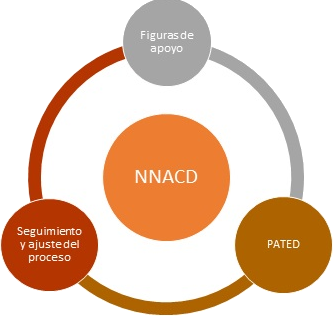
\includegraphics[width=0.65\textwidth]{Figura 1.png}
 \caption{Estructura del proceso PCP.}
 \label{fig01}
 \source{Adaptaciones de los autores.}
\end{figure}

\subsection{Metodología}\label{sec-normas}
Para conocer e intervenir, en función de las necesidades de accesibilidad al equipamiento tecnológico según la diversidad funcional de los estudiantes de Fe y Alegría, se utilizó la investigación de tipo cualitativa, con el fin de contar con una aproximación exploratoria del fenómeno estudiado \cite{hernandez_sampieri_metodologiinvestigacion_2014}. La metodología se planteó para conocer las aplicaciones para la accesibilidad al aprendizaje, descritas mediante la planificación centrada en la persona (PCP), con estrategias basadas en valores y en el empoderamiento de las personas con discapacidad, para ayudarlas a construir su propio proyecto de vida, que tienda a la plenitud y la felicidad.

Por tanto, se analizaron las necesidades de accesibilidad a equipamiento tecnológico que facilite la participación, comunicación y aprendizaje de los 212 NNACD, que presentan discapacidad psicosocial, intelectual, múltiple, síndrome de Down, síndrome de West, trastorno del espectro autista, discapacidad física, parálisis cerebral infantil y retraso madurativo en el desarrollo.

El diagnóstico se realiza tomando en cuenta a los 212 NNACD de las Unidades Educativas que son parte de este estudio, en general se analiza el grado de discapacidad que presentan. El escenario ideal, en cuanto a terminología, podría manejarse según lo describen los factores personales categorizados por la Clasificación Internacional del Funcionamiento de la Discapacidad y de la Salud (2001), en la que se detallan a discapacidad nula, leve, moderada, grave y muy grave. La base de datos refleja que en discapacidad leve hay un 2,36\% de NNACD, moderada un 22,17\%, grave un 13,21\% y muy grave un 14,15\%. Adicionalmente, se manejan otras descripciones:  discapacidad profunda 21,70\%, severa 16,51\%, sin discapacidad 0,47\%; el 9,43\% de los NNACD no definen su discapacidad.

Las cifras reflejan la necesidad imperante de proponer un plan de accesibilidad tecnológica y funcional para los NNACD, especialmente en los casos de discapacidad moderada y profunda que son los predominantes. Complementariamente, los datos son analizados por cada una de las instituciones educativas.

\section{Resultados}\label{sec-conduta}
Para comprender el contexto de cada una de las instituciones educativas, respecto a la atención a las necesidades educativas de los NNACD, así como las necesidades de accesibilidad, se consideró la Ruta de Atención a la Diversidad, descrita en la Guía Metodológica para la Atención Educativa a la Diversidad de \textcite{fe_y_alegria_guimetodologica_2020}, la que orienta en la forma de recopilar información, según la oferta de cada una de las instituciones educativas. A manera de ejemplo se evidencia a la Unidad Educativa Especial 4, pues cuenta con una mayor cantidad de NNACD, siendo 105, de entre 5 a 21 años de edad, que pertenecen a los niveles de educación inicial (niños de 3 a 4 años y de 4 a 5 años) y educación general básica (EGB). Cabe aclarar que, en la base de datos, no se detallan todas las edades de los niños y niñas del nivel inicial. El nivel inicial está conformado por un aula especial con 3 niñas y 2 niños, Solo se conoce el tipo de discapacidad de dos de ellas. La \Cref{tab01} muestra el tipo de discapacidad de la institución educativa referida. 

\begin{table}[h!]
\centering
\begin{threeparttable}
\caption{Tipo de discapacidad de la Unidad Educativa Especial 4 (Aula especializada).}
\label{tab01}
\centering
\begin{tabular}{l S S[table-format=3.2]}
\toprule
Tipo de discapacidad & {Estudiantes} & {\si{\percent}} \\
\midrule
Intelectual & 83 & 79,04  \\
Intelectual Física & 4 & 3,80   \\
Multidiscapacidad & 13 & 12,26  \\
Parálisis Cerebral Infantil & 1 & 0,94  \\
Síndrome de West & 1 & 0,94  \\
Otros & 3 & 2,85 \\
Total de estudiantes & 105 & 100  \\
\bottomrule
\end{tabular}
\source{Recopilación de los autores.}
\end{threeparttable}
\end{table}

A continuación, se evidencia la información organizada en tres niveles con el fin de presentar datos relacionados con equipos y conectividad, psicomotricidad de los NNACD y entrega pedagógica, según información tomada por docentes, basada en los mapeos e información obtenida específicamente para este estudio.

\subsection{Nivel 1: Equipos y conectividad}\label{sec-fmt-manuscrito}
En la Unidad Educativa Especial 4, tomada como ejemplo, la mayoría de NNACD cuentan con equipos que podrían facilitar las actividades de aprendizaje funcional. 19 estudiantes señalan que utilizan como recursos celulares inteligentes, así como televisores de última generación; estos equipos podrían facilitar las actividades de aprendizaje funcional en cierta medida. La \Cref{tab02} detalla el equipamiento tecnológico.

\begin{table}[h!]
\centering
\begin{threeparttable}
\caption{Equipamiento tecnológico en los hogares de los NNCD.}
\label{tab02}
\centering
\begin{tabular}{l S}
\toprule
Equipamiento & {Cantidad} \\
\midrule
Celular (inteligente) & 4   \\
Computador de escritorio & 30  \\
Portátil (laptop) & 29 \\
Sin información & 3 \\
Tableta & 24 \\
Televisor de última generación & 15 \\
Total & 105 \\
\bottomrule
\end{tabular}
\source{Recopilación de los autores.}
\end{threeparttable}
\end{table}

En relación al acceso a la conectividad en los hogares se muestra la \Cref{tab03}.

\begin{table}[h!]
\centering
\begin{threeparttable}
\caption{Acceso a conectividad en los hogares de los NNCD de la Unidad Educativa Especial 4.}
\label{tab03}
\centering
\begin{tabular}{l S}
\toprule
Conectividad & {Cantidad} \\
\midrule
Sin información & 3 \\
Wi-Fi (datos fijos) & 102  \\
Total & 105 \\
\bottomrule
\end{tabular}
\source{Recopilación de los autores.}
\end{threeparttable}
\end{table}

\subsection{Nivel 2: Psicomotricidad de los NNACD}\label{sec-formato}
\textit{En relación al manejo de la pantalla táctil (tableta)}

Como alternativas se describieron: tiene habilidades motrices para usar la pantalla táctil de la tableta; señala, sin dificultad y manteniendo el control, cualquier elemento de la pantalla; señala, con mucha dificultad, algunos elementos de la pantalla y/o no puede señalar ningún elemento de la pantalla. De los 41 NNACD, que refiere esta información, solo 7 mencionan tener habilidades motrices para usar la pantalla táctil de una tableta; 5 describen tener dificultades. Sin embargo, 26 NNACD describen más de una opción. La \Cref{fig02} evidencia lo señalado.

\begin{figure}[h!]
 \centering
 \includegraphics[width=0.85\textwidth]{Gráfico 1.png}
 \caption{Población que refiere ejecutar acciones relacionadas con el uso de pantallas táctiles.}
 \label{fig02}
 \source{Recopilación de los autores.}
\end{figure}

\textit{Manejo del cursor (apuntador)}

Como alternativas se describió lo siguiente: Los NNACD pueden apuntar íconos en la pantalla táctil con un dedo (tap), pueden ejecutar la acción de doble click con un dedo (doble tap), pueden mantener presionado un ícono durante dos segundos con un dedo, pueden arrastrar y soltar íconos de la pantalla táctil y pueden hacer uso de la pinza digital para ampliar o reducir imágenes. Las opciones planteadas han sido respondidas por 35 NNACD, de quienes se muestra: 1 persona puede hacer uso de la pinza digital para ampliar o reducir imágenes, 1 persona puede mantener presionado un ícono durante dos segundos con un dedo, 6 personas pueden apuntar íconos en la pantalla táctil con un dedo (tap) y 27 personas pueden ejecutar más de 2 alternativas.

Por lo señalado, si bien los NNACD hacen ciertos movimientos con los dedos, dan paso a que el cerebro emita respuestas motrices, obteniendo como resultado el desarrollo de su creatividad y desenvolvimiento ante ciertos estímulos \cite{puertas_motricidad_2017}. Por tanto, se debe fortalecer la aplicación de ciertos movimientos o impulsos a nivel de las extremidades superiores, como procesos madurativos, cognitivos y motrices relacionados con la coordinación óculo-manual, para lograr la precisión de movimientos controlados, siendo un aporte para las acciones de touch; sin embargo, constituye una dificultad para la accesibilidad según los datos descritos: únicamente el 18,03\% señaló poder hacerlo solo. Ante esto y tomando en cuenta las diferentes discapacidades de los NNACD, se podría hacer uso de punteros cefálicos (dispositivo que permite el control de diferentes elementos mediante los movimientos del cuello), licornio (permite el control de diferentes elementos mediante la cabeza), ratones magnificados (permiten el acceso mediante el ratón a usuarios que, aun teniendo posibilidad de usar ratones convencionales, no disponen de precisión en el movimiento), ratones de bola (permiten utilizar el computador con el puntero del ratón con los movimientos de la bola), ratones de tipo Joystic (para personas con discapacidad física, para lesión medular, esclerosis múltiple, enfermedades neuromusculares, parálisis cerebral, daño cerebral, traumatismo craneoencefálico), pad mouse (está dirigido a aquellas personas con dificultades motoras), Enable viacam (sustitutivo del ratón que mueve el puntero a partir de movimientos de la cabeza), entre otros.

\textit{Uso del teclado}

Como alternativas se describieron: puede escribir sin ninguna dificultad en el teclado, presiona diversas teclas simultáneamente sin desearlo, presiona repetidamente una tecla sin desearlo y le cuesta dejar de hacerlo antes de presionar la siguiente. Responden 63 NNACD; las opciones planteadas muestran que 23 personas presionan diversas teclas simultáneamente sin desearlo, a 2 personas les cuesta dejar de presionar una tecla antes de pasar a la siguiente, 9 personas presionan repetidamente una tecla sin desearlo y 2 personas pueden escribir sin ninguna dificultad en el teclado; sin embargo, 27 personas han señalado más de dos opciones.

Lo que muestra que el uso del teclado no sería una alternativa para los NNACD respecto al equipamiento, pues su uso no es el óptimo. Se podría hacer uso de equipos complementarios como el pulsador de teclas, un elemento que permite operar teclados de computadoras, calculadoras, teléfonos, etc.

\textit{Visualizar la pantalla del equipo}

Como alternativas se describieron: tiene dificultad para visualizar la pantalla, se acerca demasiado a la pantalla, distingue los colores de los elementos de la pantalla y visualiza el texto que aparece en la pantalla. Responden 96 NNACD; las opciones planteadas muestran que 15 personas distinguen los colores de los elementos de la pantalla, 15 personas visualizan el texto que aparece en la pantalla, 21 personas se acercan demasiado a la pantalla y 3 personas tienen dificultades para visualizar la pantalla, mientras que 42 personas han seleccionado más de dos opciones.

Lo que muestra que la pantalla de cualquier equipo de cómputo se puede visualizar con ciertas restricciones, pero es posible su uso. Muy pocas personas han referido dificultades para visualizar la pantalla, para este grupo en cierta medida se ratifica lo mencionado por el estudio realizado por \textcite{acosta-vargas_accessibility_2021} casi ninguna aplicación es 100\% accesible para una persona con discapacidad, siendo una dificultad el contraste de imagen (visual).

\textit{Puede escuchar los sonidos del equipo con el que trabaja}

Como respuesta se describieron, 9 NNACD tienen dificultad para escuchar el sonido de la música o video, 9 personas se acercan demasiado al equipo para escuchar y 70 personas escuchan normalmente, además 4 personas han señalado más de una opción.

Lo que muestra que el equipamiento tecnológico deberá contar con herramientas que faciliten la audición. Casi la totalidad de NNACD podrán hacer uso de aplicaciones informáticas que incluyen audio.

\textit{Uso de la voz para controlar el equipo}

Como respuesta se describió: 17 NNACD tienen un habla perfectamente entendible como para dar órdenes al equipo, 41 personas emiten sonidos difíciles de entender, 14 no emiten sonidos y 1 persona se acerca demasiado al equipo para escuchar, además 5 personas han seleccionado más de una opción.

Lo que muestra que los NNACD en su mayoría tienen ciertas dificultades para escuchar, el uso de aplicaciones informáticas en un 100\% es accesible para las personas que presenten discapacidades \cite{acosta-vargas_accessibility_2021}.

\textit{Uso de sistemas alternativos y aumentativos de comunicación (SAAC)}

El uso de SAAC muestra que 23 personas se comunican con lenguaje de señas, 5 personas se comunican por medio de un set de pictogramas hechos en papel/cartulina y 4 señalan no necesitar SAAC; sin embargo, 25 personas describen hacer uso de más de dos opciones.  

Lo que implica que, si bien los NNACD hacen uso de sistemas alternativos y aumentativos de comunicación (principalmente el lenguaje de señas), se pueden utilizar otros recursos como pictogramas. Tomando en cuenta la presente propuesta del PATED se sugiere hacer uso de aplicaciones informáticas relacionadas con la utilización de pictogramas temáticos según la edad, se podría organizar los temas tomando en cuenta una categorización por grupos: i) niños y niñas y ii) adolescentes.

\subsection{Nivel 3: Entrega pedagógica}\label{sec-modelo}
\textit{Autonomía de los NNACD}

Como respuesta 72 NNACD señalan más de dos opciones respecto a la autonomía en la movilidad, en la alimentación, en la higiene y en la vestimenta. Se aclara que se encontraron observancias que ciertos NNACD ejecutan estas acciones con ayudas. La \Cref{fig03} evidencia lo señalado.

\begin{figure}[h!]
 \centering
 \includegraphics[width=0.85\textwidth]{Gráfico 2.png}
 \caption{Autonomía.}
 \label{fig03}
 \source{Recopilación de los autores.}
\end{figure}

\textit{Personas que apoyan a los NNACD}

Como respuesta se describió el apoyo de la familia, principalmente se señala a las mamás, pero también a los papás, hermanos o familiares cercanos como abuelos y tíos; tutores y terapistas. 208 NNACD han referido esta información, que ha sido tomada de otra base de datos, en la que han indicado el apoyo principalmente de la familia. Del total de informantes, 120 señala a la familia, 24 señala requerir el apoyo de la familia y tutores, 27 describe a la familia, tutores y terapistas y 37 señala requerir el apoyo de la familia, terapistas y tutores.

Los datos permiten inferir que los NNACD tienen dependencia principalmente de la familia, aunque algunos también requieren el apoyo de terapistas y para los aprendizajes han señalado ayuda de sus tutores. Esto implica que, para el uso de los equipos electrónicos, así como de diferentes aplicaciones, deberán conocer sobre su uso los padres de familia y los tutores.

\textit{Estilos de aprendizaje}

Los estilos de aprendizaje han sido respondidos por 62 personas, mayoritariamente señalan los aprendizajes basados en el aspecto visual, auditivo, kinestésico, musical y aprendizaje en la naturaleza, o han descrito más de dos estilos de aprendizaje. Los NNACD en su mayoría indican no saber leer ni escribir.

Lo señalado permite inferir que los NNACD podrán desarrollar sus aprendizajes funcionales, basados en actividades lúdicas o en ramas artísticas como la música, danza, teatro, artes plásticas o literatura, lo que podrá ser complementado con el apoyo de aplicaciones informáticas que permitan fomentar el uso de gamificaciones y el arte. Para \textcite{borja_arte_2013}, en casos de estudiantes con discapacidad, las artes son un gran aporte para su desenvolvimiento apropiado, ya que no solo les brindan gran diversión, sino que pueden proveer grandes beneficios para el desarrollo de las áreas en las que tengan dificultad, lo que es ratificado por el \textcite{ministerio_de_educacion_curriculo_2006}MINISTERIO DE EDUCACIÓN, (2016, p. 50) “la cultura y las artes contribuyen a que nuestras vidas sean más plenas en todos los sentidos, generando una parte significativa del capital intelectual y creativo, personal y social”.  

\textit{Neurodidáctica para el aprendizaje de los NNACD basadas en la accesibilidad tecnológica}

La neurodidáctica, analizada como una rama de la pedagogía, basada en los planteamientos de la neurociencia, permite dar nuevas orientaciones a la educación. Busca el desarrollo de estrategias didácticas y metodológicas más eficientes, para promover un desarrollo cerebral en términos que los educadores puedan interpretar. Busca dar respuesta a la diversidad de las necesidades educativas, es decir, desde el enfoque propuesto por la educación inclusiva, creando sinapsis, enriqueciendo el número de conexiones neurales, su calidad y capacidades funcionales; mediante interacciones, se podrá desarrollar desde edades muy tempranas y durante toda la vida \cite{paniagua_g_neurodidactica:_2013}. Por tanto, el análisis y valoración de los diferentes RTED, permitirá a los NNACD el desarrollo de competencias motrices basadas en un aprendizaje funcional, con el fin de lograr la accesibilidad tecnológica tomando en cuenta el uso eficiente de equipos electrónicos como tabletas y el uso de aplicaciones informáticas.

A continuación, se realiza una descripción general, así como precisiones respecto a ciertas discapacidades con el fin de lograr diferenciaciones sutiles. Amerita recomendar que se busca lograr una autonomía muy sutil en los NNACD, basada en el establecimiento de rutinas en actividades psicomotoras finas, discriminación visual y auditiva, y coordinación viso manual.

\textit{Para los NNACD}

\begin{itemize}
    \item  Realizar el agarre de objetos, utilizar el índice para señalar o tingar objetos.
    \item Realizar la pinza índice y pulgar.
    \item Tener coordinación visual con objetos y con la mano.
    \item Tener buena disociación hombro, codo, antebrazo, muñeca y dedos.
    \item Realizar la pinza con los dedos índice y pulgar (trípode), con el fin de lograr abrir y cerrar la pantalla.
    \item Discriminar ruidos y sonidos.
    \item Responder o expresar satisfacción o insatisfacción frente a los estímulos.
    \item Centrar la mirada.
    \item Seguir objetos que tienen luces y brillos.
    \item Expresar placer o displacer ante estímulos visuales y auditivos.
    \item Entender órdenes sencillas.
    \item Tener control postural.
    \item Desarrollar estímulos para realizar las actividades de aprendizaje funcional.
\end{itemize}
    
Las competencias descritas se podrán complementar con habilidades según ciertas discapacidades:

\textit{Especificaciones técnicas de los equipos}

Gracias a la comunicación con el Equipo Coordinador se pudieron conocer las características del equipo básico y se pudo asesorar frente a dos marcas potenciales de las tabletas: ALCATEL y LENOVO, como se muestra en la \Cref{tab04}.

\begin{table}[h!]
\centering
\begin{threeparttable}
\caption{Características Alcatel 3T 10.1".}
\label{tab04}
\centering
\begin{tabular}{p{0.3\textwidth} p{0.65\textwidth}}
\toprule
Fabricante & ALCATEL \\
Marca & ALCATEL \\
Producto & ALCATEL 3T 8094  \\
Origen de los equipos & EEUU \\
Vigencia o vida útil tecnológica (años) & 1 AÑO \\
Dimensiones de la pantalla & 10" \\
Resolución de la pantalla & 1280*800 \\
Características de la cámara principal & 5.0 MP \\
Características de la cámara frontal & 2.0 MP \\
Memoria RAM & 2 GB \\
Disco duro & 32 GB \\
Lector de tarjetas & 128 GB \\
Sistema operativo & ANDROID 9.0 PIE \\
Bluetooth & 4.2 \\
Conectividad & 4G CAT 4 ENLACE DESCENDENTE DE 150 MBIT/S ENLACE ASCENDENTE DE 50 MBIT WIFI 802.11 A/B/G/N \\
Redes & 4G PARA DATOS \\
Batería & 4080 mAh (típico)/5500mAh \\
Estuche Case anti golpes  & SI \\
Mica de vidrio & SI \\
Bluetooth Keyboard Case & SI \\
Tarjeta Externa Micro SD  & SI \\
Enlace Amazon & Alcatel 3T 10.1" \\
Costo en EEUU & US\$ 187.99 \\
\bottomrule
\end{tabular}
\source{Recopilación de los autores.}
\end{threeparttable}
\end{table}

Recursos tecnológicos para estudiantes con discapacidad. Programas a ser utilizados por los NNACD

Desde inicios de la pandemia, al cambiar la forma de trabajo, se hicieron visibles los problemas de los estudiantes, de manera particular de aquellos que tienen alguna discapacidad; lo mismo ocurrió con los docentes, al no conocer de herramientas tecnológicas para trabajar de forma virtual.

Esta realidad que se vivió tiene resultados positivos y negativos. Como algo positivo se puede citar que esta pandemia ha sido una oportunidad tanto para los docentes como estudiantes, ha permitido buscar estrategias y metodologías de aprendizaje y enseñanza. Entre los negativos están la desvinculación del sistema educativo, el alejamiento del nuevo conocimiento y el rompimiento de su relación con los compañeros y docentes. El presente PATED tiene como objetivo identificar las diferentes aplicaciones tecnológicas afines a la educación que facilitan la vinculación entre docente, estudiante y el aprendizaje, enfocadas en las competencias para los 212 NNACD. La \Cref{tab05} (\Cref{apx-caract}) contiene una caracterización de programas según el tipo de discapacidades.


\textit{Apoyos técnicos para uso tecnológicos de los NNACD}

Es importante complementar el apoyo tecnológico con equipamiento electromecánico para los casos severos de parálisis cerebral, estos apoyos se resumen en la \Cref{tab06}.

\begin{table}[h!]
\centering
\begin{threeparttable}
\caption{Apoyos tecnológicos con equipamiento electromecánico.}
\label{tab06}
\centering
\begin{tabular}{p{0.2\textwidth} p{0.51\textwidth} p{0.2\textwidth}}
\toprule
EQUIPO & DESCRIPCIÓN & ENLACE \\
\midrule
GlassOuse & Par de gafas para controlar el puntero del ratón; se conecta a teléfonos móviles, ordenadores, tabletas y televisores inteligentes a través de Bluetooth para facilitar el uso de la tecnología a personas con movilidad restringida & www.amazon.com \\
Soporte para Tableta & Soporte para montaje en brazo de tableta, soporte de interruptor de Nintendo con brazo de aluminio resistente para iPad, iPad Air, iPhoneX, iPhone 8/7, Samsung Galaxy & www.amazon.com \\
Viozon & Soporte para tablet (rotación de 360 grados, flexible, altura y ángulo ajustable, aleación de aluminio de alto grado compatible con teléfono móvil y tableta 4.5-13, iPhone, iPad (blanco) & www.amazon.com \\
AbleNet BIGtrack 2.0 Trackball Mouse & Ratón para personas con discapacidad limitada & www.amazon.com \\
Tobii Eye Tracker 5 & Seguidor de ojos para mover el ratón en un computador & www.amazon.com \\
Runshuangyu & Control de pedal con interruptor de acción de un solo pie, controlador de pedal, compatible con personas con discapacidad que utilizan el teclado HID para ordenador, ratón, ordenador portátil & www.amazon.com \\
ZALU & Lápiz óptico para pantallas táctiles & www.amazon.com \\
AWAVO & Lápiz capacitivo para iPad para todas las edades, compatible con iPads y iPhone, tabletas capacitivas de pantalla táctil, smartphones & www.amazon.com \\
\bottomrule
\end{tabular}
\source{Recopilación y aplicación de los autores.}
\end{threeparttable}
\end{table}

\section{Conclusiones}\label{sec-organizacao}
Las instituciones educativas de este estudio cuentan con 212 NNACD, de quienes se detalla el grado de discapacidad que presentan. Es importante tomar en cuenta la terminología según lo describe la Clasificación Internacional del Funcionamiento de la Discapacidad y la Salud (2001) en la que se clasifica a las discapacidades según: i) funcionamiento y discapacidad: funcionamiento y estructura corporal, y actividades y participación y ii) factores contextuales: factores ambientales y factores personales. Por tanto, los términos relacionados con el tipo de discapacidad se podrían modificar. Además, es importante tomar en cuenta que 9 NNACD no han definido su discapacidad, para ellos sería importante proponer medidas de apoyo.

Los datos se desarrollan en tres niveles, no solo permiten indagar sobre los conocimientos de las TIC en el ámbito global respecto a su utilización, sino que permitirán definir las diferentes competencias que asumen los NNACD según discapacidades específicas y respecto a la accesibilidad tecnológica.

Tomando en cuenta el primer nivel relacionado con equipamiento y conectividad: i) Equipamiento electrónico: los datos dan una idea del escenario sobre el equipamiento electrónico para acceder al servicio educativo durante esta emergencia sanitaria con un 94,81\% respecto a la totalidad de la población. Las cifras reflejan que principalmente los NNACD hacen uso de tabletas, seguido de celulares inteligentes (sin ser de uso exclusivo) y muy pocos cuentan con una computadora de escritorio. ii) Equipamiento y conectividad: se evidencia que el 77,35\% equivalente a 164 NNACD se conectan con el servicio de Wifi en el hogar, en menor porcentaje se ve el acceso a un plan de datos móviles o con recargas. iii) Formas de hacer uso de equipos electrónicos: la mayoría de NNACD señala requerir ayuda para encender el equipo, muy pocos refieren que lo pueden hacer solos; como acciones pueden subir y bajar el volumen, mientras que situaciones específicas como aumentar y disminuir el brillo de la pantalla o conectarse y desconectarse al internet, lo hacen muy pocos.

Los principales recursos utilizados son tabletas, celulares inteligentes y computadoras. El uso de las computadoras de escritorio permite un mayor campo de trabajo, especialmente en estudiantes con discapacidad intelectual y parálisis cerebral infantil, ya que requieren adaptaciones tecnológicas adicionales, como teclados, pantallas, cámaras y/o ratones; sin embargo, sus costos resultan ser más elevados. Las tabletas son una alternativa de mayor accesibilidad en cuanto a costos; una tableta según su capacidad podría costar entre \$80 y \$150; sin embargo, amerita analizar su uso en cuanto a factores relacionados con lo táctil. Hay que tomar en cuenta las necesidades de cada uno de los usuarios. Para \textcite{acosta-vargas_accessibility_2021} casi ninguna aplicación es 100\% accesible para una persona con discapacidad, las dificultades de mayor accesibilidad a los equipos lo constituyen el ‘touch’ y el contraste de imagen (visual), aunque también está la dificultad del audio.

El segundo nivel relacionado con equipamiento y conectividad: i) Manejo de la pantalla táctil (tableta): muy pocos NNACD han desarrollado la habilidad de usar la pantalla táctil; lo que amerita, de una manera muy sutil, desarrollar las habilidades motrices con el fin de lograr su uso. ii) Manejo del cursor apuntador: muy pocos niños hacen uso efectivo del cursor (18,03\%). Al fusionar estos dos numerales se muestra que las acciones de touch son una dificultad para la accesibilidad, lo que ratifica la necesidad de apoyos. iii) Uso del teclado: en la mayoría de NNACD no es una alternativa respecto al equipamiento, pues su uso no es el óptimo. iv) Visualizar la pantalla del equipo con el que trabaja: su uso es posible, pero con restricciones. v) Escuchar los sonidos del equipo con el que trabaja: la mayoría tienen ciertas dificultades para escuchar. vi) Uso de sistemas alternativos y aumentativos de comunicación: principalmente hacen uso de lenguaje de señas, que puede ser algo natural; sin embargo, se podrían usar pictogramas temáticos según la edad, organizando los temas por categorías para niños, niñas y adolescentes.

El tercer nivel relacionado con entrega pedagógica: i) Autonomía para ciertas funciones: movilidad, alimentación, higiene y vestimenta; sin embargo, hay quienes señalan que únicamente tienen movilidad o alimentación o higiene o se visten autónomamente. ii) Demanda de apoyo de la familia, tutor y terapista, quienes principalmente tienen dependencia con la familia, aunque algunos también requieren el apoyo de terapistas y para los aprendizajes, han señalado ayuda de sus tutores. iii) Desarrollo de los aprendizajes: han descrito funciones como visuales, auditivos, kinestésicos, apoyo de la música y estar en contacto con la naturaleza.

Lo relacionado con el aprendizaje funcional permite inferir que los NNACD, si bien tienen ciertas autonomías, dependen de la ayuda de un familiar para lograr el aprendizaje funcional; se recomienda hacer uso de aplicaciones que fomenten las actividades lúdicas o en ramas artísticas como música, danza, teatro, artes plásticas o literatura.

La información de los mapeos familiares analizados es un insumo muy valioso, ya que se puede profundizar en las condiciones en las que viven las familias de NNACD, en especial conocer fortalezas, gustos, desagrados, sueños, temores y días especiales de los estudiantes; que constituyen actividades complementarias a las académicas, muy necesarias para generar un ambiente de armonía en su proceso de formación.

Los NNACD deberán desarrollar competencias motrices de aprendizajes, basadas en la accesibilidad tecnológica. De manera general tienen que realizar el agarre de objetos, utilizar el índice para señalar o tingar objetos, hacer la pinza índice y pulgar, coordinar la mano y la vista para tomar objetos, centrar la mirada, seguir con la mirada objetos con luces y brillos, expresar placer o displacer ante estímulos visuales y auditivos, entender órdenes sencillas, tener control postural y desarrollar estímulos para realizar las actividades de aprendizaje funcional. Estas competencias se complementan con precisiones para algunas discapacidades como multidiscapacidad, trastorno del lenguaje, síndrome de Down, trastorno del espectro autista, discapacidad intelectual y parálisis cerebral.

Los RTED son una referencia al hacer uso del equipamiento y apoyos tecnológicos específicos de los equipos, adaptaciones y software según las diferentes necesidades educativas presentadas por los NNACD; y son un insumo que orientó el equipamiento tecnológico según las necesidades educativas especiales asociadas a la discapacidad, relacionadas con discapacidad intelectual, parálisis cerebral infantil, multidiscapacidad, síndrome de Edwards, discapacidad sensorial y síndrome de Down.

Finalmente la neurodidáctica, en este estudio garantiza la implementación de estrategias didácticas y metodológicas más eficientes, para promover un desarrollo cerebral en términos que los educadores puedan interpretar, pues el análisis y valoración de los diferentes RTED, permitirá a los NNACD el desarrollo de competencias motrices basadas en un aprendizaje funcional, con el fin de lograr la accesibilidad tecnológica tomando en cuenta el uso eficiente de equipos electrónicos como tabletas y el uso de aplicaciones informáticas.

\printbibliography\label{sec-bib}
% if the text is not in Portuguese, it might be necessary to use the code below instead to print the correct ABNT abbreviations [s.n.], [s.l.]
%\begin{portuguese}
%\printbibliography[title={Bibliography}]
%\end{portuguese}


%full list: conceptualization,datacuration,formalanalysis,funding,investigation,methodology,projadm,resources,software,supervision,validation,visualization,writing,review
\begin{contributors}[sec-contributors]
\authorcontribution{Karina Delgado Valdivieso}[conceptualization,methodology,validation,writing,review]
\authorcontribution{Janio Jadán Guerrero}[methodology,validation,writing,review]
\end{contributors}

\appendix
\section{Caracterización de programas}\label{apx-caract}

%\afterpage{%
\setlength\LTleft{-1in}
\setlength\LTright{-1in}
\begin{small}
\begin{longtable}{
    p{0.1\textwidth}
    p{0.3\textwidth}    
    p{0.7\textwidth}    }
\caption{Caracterización de programas por tipo de discapacidad.}
\label{tab05}
\\
\toprule
TIPO DE DISCAPACIDAD & APLICACIÓN SOFTWARE HARDWARE & DESCRIPCIÓN \\
\midrule
\parbox[t]{2mm}{\multirow{8}{*}{\rotatebox[origin=c]{90}{Psicosocial}}} & MEFACILYTA AMIALCANCE & Forman parte de la comunidad Conectados por la Accesibilidad, y proporciona un entorno de configuración de distintos barridos de pantalla, siendo los principales barridos, los barridos por componentes, de barras y facial \\
  & SPEEDSTAR & Juego basado en una carrera de coches, en la que el usuario debe conseguir monedas y salvar obstáculos. Además posibilita competir con otro jugador, lo que favorece la interacción y la participación social de las personas con discapacidad  \\
  & COMUICANT & Utilizada por personas con problemas de habla (disartria o afasia). El programa permite convertir lo que se dicte con la voz en un texto y facilitar la comunicación entre personas con diferentes discapacidades. \\
  & ABC COMMUNICATOR & Plataforma de comunicación que tiene una interfaz fácil de usar \\
  & PICTO TEA & Diseñada también para los niños con TEA (Trastorno del Espectro Autista), que podrán comunicarse mediante imágenes en un solo lugar, también se los puede personalizar, su reproducción es en altavoz con 6 niveles de dificultad. \\
  & OTSIMO | JUEGOS DE EDUCACIÓN ESPECIAL PARA NIÑOS & Permite el desarrollo de inteligencia lingüístico verbal, habilidades cognitivas y de aprendizajes instrumentales, desarrollada para personas diagnosticadas con trastornos y discapacidades del aprendizaje, déficit de atención, autismo, síndrome de Down, Asperger, dislexia y otras necesidades especiales. \\
 & TERAPIA DEL LENGUAJE Y COGNITIVA CON MITA & Utilizada en terapias de idioma que favorecen la lectura o el habla de niños con autismo \\
 & AUTISMO IMAGEN DISCUSIÓN & Sistema de comunicación alternativa (CA), con el fin de recuperar la capacidad de comunicación. Los sistemas de CA, puestos al servicio de la logopedia, cumplen el objetivo de ayudar al desarrollo de la comunicación y del lenguaje cuando estas funciones están alteradas por causas sensoriales, físicas o psíquicas. \\
\midrule
\parbox[t]{2mm}{\multirow{7}{*}{\rotatebox[origin=c]{90}{Física}}} & EASE TOUCH & Con Ease Touch se pueden realizar todas aquellas acciones que permiten el control del dispositivo móvil mediante un sistema que captura todos los toques en la pantalla y que permite distinguir entre aquellos que son voluntarios e involuntarios, se podrán realizar la mayoría de gestos estándar para el control del dispositivo (por ejemplo, toque, doble toque, arrastrar, deslizar, pellizcar, etc.). \\
 & PUNTERO CEFÁLICO/MENTONIANO & Dispositivo que permite el control de diferentes elementos mediante los movimientos del cuello. \\
 & TOUCHMACRO PRO & Dispositivo que recibe y transfiere al ordenador toda la información de los dedos, posición en 3D, partes que lo forman (en dicha posición, cuánto miden, separación entre partes, etc.). \\
 & MOUSE4ALL PULSADOR & Utilizada por personas con discapacidad física que tengan dificultad para utilizar una pantalla táctil: parálisis cerebral, lesión medular, tetraplejia, esclerosis múltiple, ELA, Parkinson o enfermedad neuromuscular. Además, mejora la calidad de vida de las personas que lautilizan, aumentando su autonomía, privacidad y desarrollo personal. \\
 & EVA FACIAL MOUSE & Permite acceder de forma alternativa (manos libres) a las funciones del dispositivo móvil por medio del seguimiento del rostro del usuario captado a través de la cámara frontal. A partir del movimiento del rostro permite controlar un puntero en pantalla (a modo de ratón) que proporciona el acceso directo a la mayor parte de elementos de la interfaz de usuario. \\
 & JOYSTICK MOUSE ADAPTER: EMULATE MOUSE WITH GAMEPAD & Utilizada por personas con discapacidad física, para lesión medular, esclerosis múltiple, enfermedades neuromusculares, parálisis cerebral, daño cerebral, traumatismo craneoencefálico. \\
 & EASE MOUSE & Utilizada por personas con dificultades motoras. Proporciona funciones avanzadas para simplificar el uso del puntero del ratón en dispositivos Android. \\
\midrule
\parbox[t]{2mm}{\multirow{9}{*}{\rotatebox[origin=c]{90}{Intelectual}}}
 & LICORNIO & Permite el control de diferentes elementos mediante la cabeza. \\
 & TEAPP - AUTISMO Y VIDEOJUEGOS & Desarrollo de inteligencia musical. Habilidades cognitivas y habilidades de aprendizajes instrumentales, estimula la observación, atención visual y contribuye  a conseguir mayor atención y concentración, ante los sonidos que proceden del medio o a través de la estimulación de la audición y la asociación entre el sonido escuchado y una imagen. \\
 & PICTOSONIDOS & Trabaja conceptos referidos en diferentes categorías semánticas atendiendo a los sonidos que producen (onomatopeyas). \\
 & SOY VISUAL & Utiliza láminas ilustradas y fotografías para estimular el lenguaje y ayudar a personas con necesidades en la comunicación. \\
 & SKILLZ & Utilizada por personas para recoger diferentes tipos de juegos que ayudan a mejorar la memoria, entrenar el sentido de reflejo, aumentar la precisión, aumentar la velocidad, aprender la coordinación de colores. \\
 & PATHBOOKS - AUDIOLIBROS E HISTORIAS INTERACTIVAS & Permite cambiar el curso de la historia y los eventos del libro, ser el personaje principal que llega a múltiples finales creados por las decisiones tomadas. La aplicación crea una mejor de experiencia de lectura interactiva. \\
 & BEDTIME MATH & Propone retos y sencillos problemas basados en las matemáticas para resolverlos en pocos minutos. Su objetivo, es mejorar el rendimiento de los alumnos en las matemáticas. \\
 & HABÍA UNA VEZ & Audio cuentos de uso semanal. \\
 & OPUESTOLANDIA & Estimula el área cognitiva. Permite el reconocimiento de conceptos como alto, bajo, grande, chico, muchos, pocos, pesado, liviano. \\
\midrule
\parbox[t]{2mm}{\multirow{17}{*}{\rotatebox[origin=c]{90}{Parálisis Cerebral Infantil}}} & HIPSCREEN & Programa de vigilancia de movimientos de la cadera para un niño con parálisis cerebral. Es una aplicación desarrollada por médicos especialistas en parálisis cerebral. \\
 & BABY MOVES APP & Permite evaluar el movimiento general de infantes. \\
 & AMIALCANCE & Ayuda a manejar la mayoría de aplicaciones y funcionalidades de los terminales móviles a personas con distintas restricciones en la manipulación e incluso a quienes tienen deficiencias visuales o de lecto–escritura, ya que incorpora un sistema de texto y de voz. \\
 & HERMES MOBILE & Facilita la comunicación de personas con dificultades físicas y en el habla. \\
 & SPEEDSTAR & Juego basado en una carrera de coches, en la que el usuario debe conseguir monedas y salvar obstáculos. Además, permite la posibilidad de competir con otro jugador, lo que favorece la interacción y la participación social de las personas con discapacidad. \\
 & WALKIE TALKIE ONLINE VOICE COMMUNICATION & Inspirado en las aplicaciones de causa-efecto, proporciona una herramienta para la interacción continua y a distancia, accesible a la mayoría de las personas con discapacidades cognitivas, físicas y sensoriales. \\
 & EVA FACIAL MOUSE & Sustituto del ratón que mueve el puntero a partir del movimiento de la cabeza. Funciona en un computador con una webcam sin elementos adicionales. \\
 & LEO FACIL & Permite leer las obras que integra en un formato fácil, acompañando el texto escrito con dibujos, imágenes, música y animaciones, para facilitar la accesibilidad cognitiva. La aplicación tiene dos partes: obras de relevancia para su consulta en el ámbito educativo y obras para la lectura como tiempo de ocio. \\
 & SYMBOTALK - AAC TALKER & Sistema personalizable y dinámico de comunicación aumentativa y alternativa, dirigido a personas con barreras de comunicación oral o escrita. Permite al estudiante comunicarse mediante el uso de tecnología táctil y multimedia. \\
 & COMUICANT & Utilizada por personas con problemas de habla (disartria o afasia). El programa permite convertir lo que se dicte con la voz en un texto y facilitar la comunicación entre personas con diferentes discapacidades \\
 & COMUNICADOR & Potencia las fortalezas de las personas con TEA, como hábiles aprendices visuales, por la alta motivación que los dispositivos electrónicos generan.
 Funciona como un sistema alternativo y/o aumentativo del intercambio comunicativo. \\
 & PICA & Permite crear ejercicios didácticos cooperativos de tres tipos básicos: puzzle, asociación y exploración. Los ejercicios pueden ser adaptados en contenidos y en presentaciones para que sean accesibles y utilizables para personas con necesidades educativas especiales. \\
 & ABC COMMUNICATOR & Utilizada por personas para facilitar la comunicación que tiene una interfaz fácil de usar. \\
 & LEARNY PRIMARIA - 5TO GRADO & Juego que brinda a los niños con parálisis, de entre 10 y 11 años de edad que estén cursando la primaria, dinámicas de aprendizaje, de manera que sea más fácil para ellos adquirir los conocimientos. \\
 & NEUROLOGY EXAM REVIEW \& PRACTICE QUESTIONS & Utilizada por profesionales, concretamente está pensada para que pueda ser utilizada en la práctica clínica de Neurólogos y Psiquiatras \\
 & SALIVA TRACKER & Desarrollada para cuidadores, ayuda a realizar un seguimiento de cómo progresa el niño con medicación recetada por goteo. Se le pedirá que responda las preguntas de Saliva Tracker en 1 semana, 1 mes, 3 meses y 6 meses en el momento que le resulte más conveniente. \\
 & BABY STIMULATOR & Apoya a padres en términos de estimulación temprana. La app estimula el sentido visual, auditivo y táctil del niño y también fomentará la interacción mediante el tacto y la acción. \\
\midrule
\parbox[t]{2mm}{\multirow{6}{*}{\rotatebox[origin=c]{90}{Espectro Autista}}}
 & PICTOTEA & Utiliza la tecnología para la inclusión de personas con TEA facilitando así la comunicación con su entorno mediante la comunicación por pictogramas digitales en lugar de las tarjetas físicas. \\
 & AUTISMIND & Herramienta de apoyo para ayudar a padres y profesionales a trabajar las habilidades mentalistas en niños con TEA. Siguiendo una estructura organizada y definida, AUTISMIND plantea 10 temas diferentes que abordan aspectos relacionados con la Teoría de la Mente, con 6 niveles de dificultad creciente y con un total de más de 1.000 ejercicios lúdicos e interactivos. \\
 & PROCESS & Juego de memoria y reflexión, el objetivo es memorizar una secuencia de números, cada uno de ellos se asocia con una dirección. Presenta 2 niveles de dificultad y 3 tipos de ejercicios (ordenar, qué pasará y emociones). \\
 & PICTO TEA & Diseñada para que los niños con TEA (Trastorno del Espectro Autista) puedan comunicarse mediante imágenes todos en un solo lugar también se los puede personalizar, su reproducción es en altavoz con 6 niveles de dificultad. \\
 & AUTISMO - TEA TRASTORNO DEL ESPECTRO AUTISTA & Utilizada por personas que requieran o precisen interiorizarse sobre el Autismo. \\
& JADE & Estimula el desarrollo de niños autistas y con síndrome de Down. \\
\midrule
\parbox[t]{2mm}{\multirow{6}{*}{\rotatebox[origin=c]{90}{Síndrome de Down}}}
 & PRIMERO LEE & Favorece el desarrollo de inteligencia lingüístico verbal, habilidades cognitivas y de aprendizajes instrumentales: lectura global de palabra, escritura por sílabas, adquisición de vocabulario. \\
 & VIRGINIA AYUDA & Útil en el caso de discapacidades congénitas, adquiridas y / o temporales, lo que permite a través de la intervención del dispositivo en el que está instalado, crear un mensaje de voz rápido, comunicando eficazmente los problemas, las necesidades y peticiones. \\
 & AUTISPARK & Estimula y se basa en la clasificación de colecciones de objetos. Consiste en un juego que busca estimular la construcción espacial. Utiliza varios recursos: elementos en pantalla, frutas, juguetes, vajilla y útiles escolares. \\
 & SKILLZ & Recoge diferentes tipos de juegos que ayudan a mejorar la memoria, entrenar el sentido de reflejo, aumentar la precisión, aumentar la velocidad y aprender la coordinación de colores. \\
 & OPUESTOLANDIA & Estimula el área cognitiva. Permite el reconocimiento de conceptos como alto, bajo, grande, chico, muchos, pocos, pesado, liviano. \\
 & JADE & Estimula el desarrollo de niños autistas y con síndrome de Down. \\
\midrule
\parbox[t]{2mm}{\multirow{5}{*}{\rotatebox[origin=c]{90}{Visual}}}
 & LAZZUS & Asistente que acompaña a las personas ciegas y con discapacidad visual en sus desplazamientos creando un campo de visión auditivo. \\
 & LAZARILLO & Utiliza el GPS e informa de las rutas, entornos y tiendas. \\
 & TAP TAP SEE & Diseñada para iPhone y Android que ayuda a las personas ciegas o con alguna limitación visual a identificar objetos. Para utilizarla, el usuario solo tiene que hacer una foto con su móvil. La app lo identifica y provee una descripción oral mediante el lector de pantalla. \\
 & BRAILLEBACK & Permitirá utilizar un dispositivo Android con una pantalla braille. \\
 & EASY TOUCH & Rastrea el movimiento del dedo, identifica palabras y procesa la información, además. El artefacto tiene motores vibrantes que alertan al lector cuando se aparta de la línea de texto. \\
Multidiscapacidad & \multicolumn{2}{c}{Todas las aplicaciones referidas, según el tipo de discapacidad.} \\
\bottomrule
\source{Recopilación y aplicación de los autores.}
\end{longtable}
\end{small}
%}% end of scope of afterpage directive 

\end{document}

